% =====================================================================
%  Administrativo — Modulele, unul câte unul (catalog de module)
%
%  Compilare:  tectonic -X compile prezentare-module.tex
%  Motor: XeLaTeX / LuaLaTeX (fontspec). NU compila cu pdflatex.
%
%  Sora prezentării comerciale: aceeași temă (`tema/`), fără partea de
%  abonament și prețuri. Un slide pe fiecare dintre cele nouăsprezece module
%  din `src/config/features.ts`, cu captura reală din aplicație acolo unde
%  există una (`capturi/`, generate din `public/capturi/`).
%
%  DE UNDE VINE TEXTUL: din fișele de modul ale site-ului
%  (`src/content/landing/fise-module.ts`), verificate în cod. Unde fișa și
%  codul se contrazic, câștigă codul — vezi README, „Ce s-a scos din
%  prezentarea veche".
% =====================================================================
\documentclass[aspectratio=169,11pt,t,xcolor={table}]{beamer}

% =====================================================================
%  Tema Administrativo — pachetele comune, paleta de brand și tipografia.
%  Comună tuturor materialelor din docs/comercial/ (Beamer și A4).
%  Se încarcă imediat după \documentclass; cere xcolor deja încărcat
%  (beamer îl încarcă singur; un `article` îl încarcă înainte de \input).
%
%  ORDINEA CONTEAZĂ: pachetele se încarcă ÎNAINTEA fonturilor. `booktabs`
%  își fixează distanțele (\aboverulesep = 0,4ex) la încărcare, din fontul
%  curent; încărcat după TeX Gyre Heros, liniile tabelelor coborau 0,35 pt.
% =====================================================================

\usepackage{fontspec}
\usepackage{polyglossia}
\setmainlanguage{romanian}   % despărțire în silabe corectă pentru textul românesc
\usepackage{tikz}
\usepackage[most]{tcolorbox}
\usepackage{fontawesome5}
\usepackage{booktabs}
\usepackage{array}
\usepackage{ragged2e}
\usetikzlibrary{positioning,calc,arrows.meta,decorations.pathreplacing}

% ---------------------------------------------------------------------
% 1. Identitate vizuală — paleta de brand
% ---------------------------------------------------------------------
\definecolor{brandNavy}{HTML}{0E1B2E}   % fundal închis, coperți
\definecolor{brandBlue}{HTML}{2563EB}   % primar
\definecolor{brandTeal}{HTML}{0EA5A4}   % accent
\definecolor{brandAmber}{HTML}{F59E0B}  % evidențieri
\definecolor{brandGreen}{HTML}{16A34A}  % disponibil, confirmări
\definecolor{brandSlate}{HTML}{475569}  % text secundar
\definecolor{brandMist}{HTML}{F1F5F9}   % fundal cutii
\definecolor{brandLine}{HTML}{CBD5E1}   % linii, chenare fine

% ---------------------------------------------------------------------
% 2. Tipografie
% ---------------------------------------------------------------------
\defaultfontfeatures{Ligatures=TeX}
\setsansfont{texgyreheros}[Extension=.otf,UprightFont=*-regular,
  BoldFont=*-bold,ItalicFont=*-italic,BoldItalicFont=*-bolditalic]
\setmainfont{texgyreheros}[Extension=.otf,UprightFont=*-regular,
  BoldFont=*-bold,ItalicFont=*-italic,BoldItalicFont=*-bolditalic]
\newfontfamily\titlufont{texgyreadventor}[Extension=.otf,UprightFont=*-regular,
  BoldFont=*-bold,ItalicFont=*-italic,BoldItalicFont=*-bolditalic]

% =====================================================================
%  Tema Beamer Administrativo — șabloane și componente.
%  Se încarcă DUPĂ tema/baza.tex. Folosită de prezentare-comerciala.tex
%  și de prezentare-module.tex: un slide nou = un apel de macro, nu un
%  preambul copiat.
% =====================================================================

% ---------------------------------------------------------------------
% 3. Tema beamer — construită de la zero, fără ornamentele implicite
% ---------------------------------------------------------------------
\usetheme{default}
\setbeamertemplate{navigation symbols}{}
\setbeamercolor{normal text}{fg=brandNavy,bg=white}
\setbeamercolor{structure}{fg=brandBlue}
\setbeamersize{text margin left=0.85cm, text margin right=0.85cm}
\setbeamertemplate{itemize item}{\mbox{\textcolor{brandBlue}{\footnotesize\faIcon{caret-right}}}}
\setbeamertemplate{itemize subitem}{\mbox{\textcolor{brandTeal}{\scriptsize\faIcon{minus}}}}
\setlength{\parskip}{0pt}
% Măsură scurtă peste tot (coloane de 4–8 cm): aliniere la stânga, cu despărțire
% în silabe. Textul justificat lasă găuri urâte pe rânduri atât de scurte.
\AtBeginDocument{\RaggedRight}

% Titlu de slide: titlu gros + linie de accent
\setbeamertemplate{frametitle}{%
  \vspace*{0.34cm}%
  \begin{minipage}{\linewidth}%
    \raggedright
    {\titlufont\bfseries\large\color{brandNavy}\insertframetitle}\par
    \vspace{3pt}
    {\color{brandBlue}\rule{1.7cm}{2.2pt}}%
  \end{minipage}%
  \vspace*{0.14cm}%
}

% Subsol: marcă, poziționare, număr de pagină
\setbeamertemplate{footline}{%
  \hbox{%
    \hspace*{0.85cm}%
    \parbox{\dimexpr\paperwidth-1.7cm\relax}{%
      \textcolor{brandLine}{\rule{\linewidth}{0.5pt}}\par
      \vspace{2pt}
      {\scriptsize\color{brandSlate}{\titlufont ADMINISTRATIVO}\hfill
       ERP administrativ, livrat ca abonament\hfill
       \textbf{\insertframenumber}}%
    }%
  }\vspace*{0.26cm}%
}

% ---------------------------------------------------------------------
% 4. Componente reutilizabile
% ---------------------------------------------------------------------

% Pastilă de status / etichetă colorată
\newcommand{\pastila}[2]{%
  \tikz[baseline=(x.base)]{\node[fill=#1,text=white,rounded corners=2.5pt,
    inner xsep=6pt,inner ysep=2.6pt,font=\bfseries\tiny] (x) {\MakeUppercase{#2}};}}

% Placă de logo — înlocuiește cu \includegraphics{sigla.pdf} când există sigla reală
\newcommand{\logoPlaceholder}[1]{%
  \begin{tikzpicture}[scale=#1,every node/.style={transform shape}]
    \draw[brandTeal,line width=1.1pt,dashed,rounded corners=6pt] (0,0) rectangle (2.6,2.6);
    \node[text=white,font=\titlufont\bfseries\LARGE] at (1.3,1.52) {A};
    \node[text=brandTeal,font=\titlufont\bfseries\tiny] at (1.3,0.62) {LOGO};
  \end{tikzpicture}}

% Card cu iconiță, titlu și text — cărămida întregii prezentări
\newtcolorbox{card}[3][brandBlue]{%
  enhanced, arc=3pt,
  colback=white, colframe=brandLine, boxrule=0.5pt,
  borderline west={2.4pt}{0pt}{#1},
  left=7pt,right=7pt,top=4pt,bottom=4pt,
  halign=flush left, halign title=flush left,
  fonttitle=\bfseries\footnotesize,
  title={\textcolor{#1}{\faIcon{#2}}\hspace{5pt}\textcolor{brandNavy}{#3}},
  colbacktitle=white, coltitle=brandNavy,
  toptitle=1pt, bottomtitle=2pt}

% Cutie de beneficii — fundal deschis, bară de accent
\newtcolorbox{beneficii}[1][Ce câștigă firma]{%
  enhanced, arc=3pt, colback=brandMist, colframe=brandTeal, boxrule=0pt,
  borderline west={3pt}{0pt}{brandTeal},
  left=8pt,right=8pt,top=4pt,bottom=4pt,
  halign=flush left, halign title=flush left,
  fonttitle=\bfseries\footnotesize, coltitle=brandTeal, colbacktitle=brandMist,
  title={\faIcon{check-circle}\hspace{5pt}#1}}

% Cutie de notă comercială evidențiată
\newtcolorbox{nota}[1][Notă]{%
  enhanced, arc=3pt, colback=brandAmber!8, colframe=brandAmber, boxrule=1pt,
  left=9pt,right=9pt,top=6pt,bottom=6pt,
  halign=flush left, halign title=flush left,
  fonttitle=\bfseries\footnotesize, coltitle=white, colbacktitle=brandAmber,
  title={\faIcon{star}\hspace{5pt}#1}}

% Cutie neutră, cu chenar întrerupt — folosită pentru placeholder-uri
\newtcolorbox{placeholder}{%
  enhanced, arc=3pt, colback=brandMist!55, colframe=white, boxrule=0pt,
  borderline={1pt}{0pt}{brandSlate,dashed},
  left=10pt,right=10pt,top=8pt,bottom=8pt}

% Rânduri de listă cu iconiță colorată.
% Fiecare rând ÎȘI ÎNCHIDE singur paragraful (\par la început și la sfârșit):
% altfel `\vspace` de deasupra rămâne în mod orizontal și rândul se lipește de
% textul dinainte. `\hangindent` aliniază continuarea sub text, nu sub iconiță.
%
% Iconița stă într-un `\makebox` de LĂȚIME FIXĂ, egală cu `\hangindent`, și e
% CENTRATĂ în el. Pictogramele Font Awesome au lățimi diferite (`user` are
% 0,875 em, `users` are 1,25 em), deci:
%   - fără casetă fixă, textul pornea din alt punct pe fiecare rând;
%   - cu casetă fixă dar aliniere la stânga, textul se alinia, dar pictogramele
%     rămâneau descentrate una față de alta.
% Alinierea e la STÂNGA, nu centrată. Centrarea pare ideea corectă, dar
% pictogramele Font Awesome au lățimi proprii diferite, deci centrate ies toate
% din altă poziție: marginea din stânga a coloanei devine zimțată, exact ce se
% vedea pe slide-ul Nucleu. Aliniate la stânga, marginile lor formează o linie
% dreaptă, iar diferența de lățime se pierde în spațiul până la text.
%
% Caseta e de 1,25 em (lățimea maximă a unei pictograme Font Awesome), iar
% spațiul până la text e ADĂUGAT SEPARAT, nu lăsat pe seama umpluturii casetei:
% altfel o pictogramă lată umple caseta și textul i se lipește, în timp ce una
% îngustă stă departe. 1,25 + 0,4 = 1,65 em, exact `\hangindent`-ul, deci
% continuarea rândului cade sub prima literă, nu sub pictogramă.
\newcommand{\randlista}[3]{%
  \par\hangindent=1.65em\hangafter=1\noindent
  \makebox[1.25em][l]{\textcolor{#1}{\faIcon{#2}}}\hspace{0.4em}#3\par}
\newcommand{\pct}[2]{\randlista{brandBlue}{#1}{#2}}
\newcommand{\pctv}[2]{\randlista{brandGreen}{#1}{#2}}

% Titlu de secțiune peste ecran plin: iconiță, titlu, subtitlu
\newcommand{\separator}[3]{%
\begin{frame}[plain]
  \begin{tikzpicture}[remember picture,overlay]
    \fill[brandNavy] (current page.south west) rectangle (current page.north east);
    \fill[brandTeal,opacity=0.10] ([xshift=-3cm,yshift=-2.4cm]current page.east) circle (5.2cm);
    \fill[brandBlue,opacity=0.16] ([xshift=-1.2cm,yshift=2.2cm]current page.east) circle (3.4cm);
    \node[anchor=west,align=left] at ([xshift=1.6cm]current page.west) {%
      \begin{minipage}{10.5cm}
        \raggedright
        {\color{brandTeal}\Large\faIcon{#1}}\par\vspace{9pt}
        {\titlufont\bfseries\huge\color{white} #2}\par\vspace{8pt}
        {\color{brandLine}\small #3}
      \end{minipage}};
  \end{tikzpicture}
\end{frame}}


% ---------------------------------------------------------------------
% 5. Tiparul unui slide de modul
% ---------------------------------------------------------------------
% Toată secțiunea de module e construită dintr-un singur macro, ca cele
% douăzeci de slide-uri să nu ajungă douăzeci de layout-uri ușor diferite.
% Un modul nou = un apel nou, nu un slide copiat și ajustat.
%
%   #1 titlul slide-ului
%   #2 grupul din meniu, tipărit ca a doua pastilă (Personal, Financiar, ...)
%   #3 paragraful de deschidere — ce e modulul, în două-trei rânduri
%   #4 funcționalitățile, ca rânduri \pct{iconiță}{text}
%   #5 beneficiile, ca rânduri \pctv{check}{text}
%
% `\vspace{-2pt}` de la început nu e cosmetic: corpul cadrului începe cu un
% grup `{...}`, iar beamer l-ar înghiți ca SUBTITLU (vezi README, capcana 1).
\newcommand{\modul}[5]{%
\begin{frame}{#1}
  \vspace{-2pt}
  {\pastila{brandGreen}{disponibil}\hspace{5pt}\pastila{brandBlue}{#2}}
  \vspace{7pt}
  \begin{columns}[T,onlytextwidth]
    \begin{column}{0.52\textwidth}
      {\footnotesize #3}
      \vspace{5pt}
      {\footnotesize #4}
    \end{column}
    \begin{column}{0.44\textwidth}
      \begin{beneficii}[Ce câștigă firma]
        \footnotesize #5
      \end{beneficii}
    \end{column}
  \end{columns}
\end{frame}}

% Card compact — doar pentru pagina cu toate modulele, unde încap opt rânduri într-o
% coloană. Aceleași culori ca `card`, dar cu jumătate din padding.
\newtcolorbox{cardm}[3][brandBlue]{%
  enhanced, arc=3pt,
  colback=white, colframe=brandLine, boxrule=0.5pt,
  borderline west={2.4pt}{0pt}{#1},
  left=6pt,right=6pt,top=1pt,bottom=2pt,
  halign=flush left, halign title=flush left,
  fonttitle=\bfseries\scriptsize,
  title={\textcolor{#1}{\faIcon{#2}}\hspace{4pt}\textcolor{brandNavy}{#3}},
  colbacktitle=white, coltitle=brandNavy,
  toptitle=0pt, bottomtitle=1pt}

% Varianta pentru un modul care ÎNCĂ NU e livrat. Singura diferență față de
% `\modul` e pastila: chihlimbar „în dezvoltare" în locul verdelui „disponibil".
% Deliberat un macro separat, nu un argument opțional: culoarea pastilei e
% singurul lucru care spune clientului că plătește pentru ceva ce încă nu poate
% folosi azi, deci nu trebuie să depindă de un parametru ușor de uitat.
\newcommand{\modulviitor}[5]{%
\begin{frame}{#1}
  \vspace{-2pt}
  {\pastila{brandAmber}{în dezvoltare}\hspace{5pt}\pastila{brandBlue}{#2}}
  \vspace{7pt}
  \begin{columns}[T,onlytextwidth]
    \begin{column}{0.52\textwidth}
      {\footnotesize #3}
      \vspace{5pt}
      {\footnotesize #4}
    \end{column}
    \begin{column}{0.44\textwidth}
      \begin{beneficii}[Ce va câștiga firma]
        \footnotesize #5
      \end{beneficii}
    \end{column}
  \end{columns}
\end{frame}}

% Celulă din pagina cu toate modulele: iconiță + denumire, pe un rând.
%
% `\tiny` se deschide ÎNAINTE de paragraf și `\par` se închide ÎN INTERIORUL
% grupului, deliberat. TeX fixează `\baselineskip` la `\par`, din mărimea
% curentă: cu `{\tiny #2}` doar pe text, literele erau mici, dar rândurile
% rămâneau la interlinia de 11pt — opt module ocupau cât un slide întreg.
\newcommand{\celula}[2]{%
  {\tiny\par\hangindent=1.6em\hangafter=1\noindent
   \makebox[1.25em][l]{\textcolor{brandBlue}{\faIcon{#1}}}\hspace{0.35em}#2\par}}

% Rând de modul cu preț: denumirea la stânga, prețul lipit de marginea dreaptă.
% `\makebox` de lățimea coloanei aduce modul LR, singurul în care `\hfill` chiar
% împinge — într-un paragraf cu `\RaggedRight` activ, glue-ul din dreapta l-ar
% fi înghițit, iar prețurile ar fi stat lipite de denumire.
\newcommand{\modulpret}[2]{%
  {\tiny\par\noindent\makebox[\linewidth][l]{#1\hfill\textbf{#2}}\par}}

% Cifră mare cu etichetă dedesubt — banda de sinteză de pe slide-ul 1.
\newcommand{\cifra}[2]{%
  \begin{minipage}[t]{3.15cm}
    \centering
    {\titlufont\bfseries\Large\color{brandBlue}#1}\par\vspace{1pt}
    {\scriptsize\color{brandSlate}#2}
  \end{minipage}}

% ---------------------------------------------------------------------
% 6. Slide de modul cu captură din aplicație
% ---------------------------------------------------------------------
% Fereastra în care stă captura: bară de titlu cu trei puncte, ca un ecran
% văzut „prin geam" — același motiv ca pe paginile de modul ale site-ului.
% Fără margine interioară: chenarul atinge imaginea, altfel captura pare
% lipită pe o foaie, nu deschisă pe un ecran.
\newtcolorbox{fereastra}{%
  enhanced, arc=3pt, colback=white, colframe=brandLine, boxrule=0.5pt,
  left=0pt,right=0pt,top=0pt,bottom=0pt, boxsep=0pt,
  halign=center,
  colbacktitle=brandMist, coltitle=brandLine,
  toptitle=1.2pt, bottomtitle=1.2pt, lefttitle=4pt,
  fonttitle=\fontsize{3.5}{4}\selectfont,
  title={\faIcon{circle}\,\faIcon{circle}\,\faIcon{circle}}}

% Banda de beneficii de sub coloane: aceleași culori ca `beneficii`, dar
% culcată pe toată lățimea, cu beneficiile pe trei coloane.
%
% De ce nu cutia `beneficii` sub captură, în coloana dreaptă: prima variantă
% așa era, și ieșea peste subsol cu 25–50 pt pe fiecare slide. Captura
% 16:10 ocupă aproape toată înălțimea coloanei; beneficiile scurte, puse în
% lat, costă un singur rând în loc de patru.
\newtcolorbox{bandabeneficii}{%
  enhanced, arc=3pt, colback=brandMist, colframe=brandTeal, boxrule=0pt,
  borderline west={3pt}{0pt}{brandTeal},
  left=8pt,right=8pt,top=3pt,bottom=4pt}

% Un beneficiu din bandă: o treime din lățime, aliniat sus. `\hfill` de la
% final împarte golul rămas între cele trei coloane.
%
% `\RaggedRight` se repune ÎN minipage: minipage reface alinierea implicită
% (`\@parboxrestore`), deci textul ieșea justificat pe o coloană de 4 cm —
% câte trei `Underfull \hbox` pe fiecare slide.
\newcommand{\benef}[1]{%
  \begin{minipage}[t]{0.27\linewidth}\RaggedRight\pctv{check}{#1}\end{minipage}\hfill}

% Același tipar ca `\modul`, cu o coloană dreaptă diferită: captura, în
% fereastră, iar beneficiile într-o bandă pe toată lățimea, dedesubt.
%
%   #1–#4 exact ca la `\modul`
%   #5    EXACT trei beneficii, ca `\benef{...}` — nu `\pctv`, și fără
%         `\par` între ele: un `\par` le-ar așeza unul sub altul
%   #6    conținutul ferestrei: de regulă `\captura{cheie}`; Portalul pune
%         aici două capturi de telefon alăturate
%
% Pastila de status NU e parametru, din același motiv ca la `\modulviitor`.
%
% Eticheta „Ce câștigă firma" stă în prima coloană a benzii, nu deasupra ei:
% pe un rând separat costa ~10 pt, exact cât ieșea banda peste subsol pe
% slide-urile cu șase funcționalități.
\newcommand{\modulcaptura}[6]{%
\begin{frame}{#1}
  \vspace{-2pt}
  {\pastila{brandGreen}{disponibil}\hspace{5pt}\pastila{brandBlue}{#2}}
  \vspace{5pt}
  \begin{columns}[T,onlytextwidth]
    \begin{column}{0.5\textwidth}
      {\footnotesize #3}
      \vspace{4pt}
      {\footnotesize #4}
    \end{column}
    \begin{column}{0.47\textwidth}
      \begin{fereastra}#6\end{fereastra}
    \end{column}
  \end{columns}
  \vspace{4pt}
  \begin{bandabeneficii}
    \scriptsize
    \begin{minipage}[t]{0.14\linewidth}\RaggedRight
      \randlista{brandTeal}{check-circle}{\bfseries\color{brandTeal}Ce câștigă firma}
    \end{minipage}\hfill
    #5
  \end{bandabeneficii}
\end{frame}}

% Captura de birou a unui modul, după cheia din `src/config/features.ts`.
% Înălțimea e plafonată, nu lățimea: capturile sunt 16:10, iar la lățimea
% coloanei ar împinge banda de beneficii peste subsol.
\newcommand{\captura}[1]{%
  \includegraphics[width=\linewidth,height=3.0cm,keepaspectratio]{capturi/#1}}


\hypersetup{
  pdftitle={Administrativo — modulele, unul câte unul},
  pdfsubject={Catalogul modulelor Administrativo, ERP administrativ pentru firme din România},
  pdfauthor={Administrativo},
  pdfkeywords={ERP, HR, module, pontaj, concedii, salarizare, REGES, SSM,
    parc auto, mentenanță, inventar, ticketing IT, portal angajat, KPI}}

\begin{document}

% =====================================================================
%  COPERTĂ
% =====================================================================
\begin{frame}[plain]
  \begin{tikzpicture}[remember picture,overlay]
    \fill[brandNavy] (current page.south west) rectangle (current page.north east);
    \fill[brandBlue,opacity=0.20] ([xshift=-2.4cm,yshift=1.7cm]current page.east) circle (4.6cm);
    \fill[brandTeal,opacity=0.14] ([xshift=-4.4cm,yshift=-2.9cm]current page.east) circle (3.1cm);
    \draw[brandTeal,opacity=0.30,line width=0.7pt]
      ([xshift=-2.4cm,yshift=1.7cm]current page.east) circle (5.7cm);
    \draw[brandBlue,opacity=0.35,line width=0.7pt]
      ([xshift=-2.4cm,yshift=1.7cm]current page.east) circle (6.6cm);

    \node[anchor=north west,text=white,font=\titlufont\fontsize{13}{15}\selectfont]
      at ([xshift=1.5cm,yshift=-1.0cm]current page.north west) {ADMINISTRATIVO};

    \node[anchor=north west,align=left] at ([xshift=1.45cm,yshift=-2.85cm]current page.north west) {%
      \begin{minipage}{11.6cm}
        \raggedright
        {\color{brandTeal}\scriptsize\titlufont\bfseries CATALOGUL MODULELOR \textperiodcentered{} 2026}\par
        \vspace{10pt}
        {\titlufont\bfseries\fontsize{26}{30}\selectfont\color{white} Modulele, unul câte unul}\par
        \vspace{12pt}
        {\color{white}\large Ce face fiecare modul —\\și ce vede omul pe ecran.}\par
        \vspace{5pt}
        {\color{brandLine}\normalsize Capturile sunt din aplicația reală, pe o firmă de demonstrație.}
      \end{minipage}};

    \node[anchor=south west,align=left] at ([xshift=1.5cm,yshift=0.95cm]current page.south west) {%
      \begin{minipage}{13.4cm}
        {\color{brandTeal}\rule{2.2cm}{2pt}}\par
        \vspace{9pt}
        {\color{white}\scriptsize
          \faIcon{th}~~Nucleu + 15 module \quad\textcolor{brandTeal}{\textbullet}\quad
          \faIcon{toggle-on}~~Pornite separat, pe firmă \quad\textcolor{brandTeal}{\textbullet}\quad
          \faIcon{mobile-alt}~~Birou și telefon}
      \end{minipage}};
  \end{tikzpicture}
\end{frame}

% =====================================================================
%  CE ESTE APLICAȚIA
% =====================================================================
\begin{frame}{Ce este Administrativo}
  \vspace{0pt}% NU șterge: fără el, beamer ia grupul {...} de mai jos drept SUBTITLU
  {\footnotesize
  Aplicația web în care se \textbf{administrează activitatea internă a unei firme din
  România}: oamenii, prezența, salariile, echipamentele și actele care le leagă —
  într-un singur sistem, cu o singură evidență. Un angajat introdus o dată apare în
  pontaj, în concedii, în salarizare și pe bunurile din primirea lui.}
  \vspace{5pt}
  \begin{columns}[T,onlytextwidth]
    \begin{column}{0.5\textwidth}
      \begin{card}[brandBlue]{users-cog}{Fiecare rol vede alt ecran}
        \footnotesize
        \pct{user-shield}{\textbf{Administratorul} — firma întreagă}\par\vspace{1pt}
        \pct{user-tie}{\textbf{Personalul} — dosare, pontaj, state}\par\vspace{1pt}
        \pct{users}{\textbf{Șeful de echipă} — oamenii lui}\par\vspace{1pt}
        \pct{user}{\textbf{Angajatul} — doar ce îl privește}
      \end{card}
    \end{column}
    \begin{column}{0.47\textwidth}
      \begin{card}[brandTeal]{flag}{Construit pe legislația românească}
        \footnotesize
        \pct{scroll}{REGES-Online, transmis din aplicație}\par\vspace{2pt}
        \pct{file-invoice}{D112 în XML și fișier de plată SEPA}\par\vspace{2pt}
        \pct{gavel}{Popriri în limitele art. 729 CPC}\par\vspace{2pt}
        \pct{calendar-day}{Pontaj în forma cerută de art. 119 CM}
      \end{card}
    \end{column}
  \end{columns}
  \vspace{5pt}
  % Fără `center`: mediul adaugă \topsep deasupra și dedesubt, iar banda de
  % cifre ieșea cu 7 pt peste subsol.
  \par\noindent
  \cifra{19}{module în total}\hfill
  \cifra{15}{opționale, peste nucleu}\hfill
  \cifra{4}{roluri, ecrane diferite}\hfill
  \cifra{0}{servere la client}
\end{frame}

% =====================================================================
%  HARTA MODULELOR
% =====================================================================
\begin{frame}{Toate modulele, pe o singură pagină}
  \vspace{0pt}% NU șterge: fără el, beamer ia grupul {...} de mai jos drept SUBTITLU
  {\scriptsize\color{brandSlate} Nucleul e mereu inclus. Celelalte cincisprezece se
  pornesc separat, pe fiecare firmă — iar paginile următoare le iau în această ordine.}
  \vspace{7pt}
  \begin{columns}[T,onlytextwidth]
    \begin{column}{0.315\textwidth}
      \begin{cardm}[brandNavy]{cube}{Nucleu — mereu inclus}
        \celula{id-card}{Nucleu: angajați, documente, registru, structură, roluri}
        \celula{clock}{Pontaj}
        \celula{calendar-alt}{Concedii}
        \celula{mobile-alt}{Portal angajat}
      \end{cardm}
      \vspace{4pt}
      \begin{cardm}[brandBlue]{infinity}{Transversal}
        \celula{magic}{Asistent AI}
      \end{cardm}
    \end{column}
    \begin{column}{0.315\textwidth}
      \begin{cardm}[brandTeal]{users}{HR extins}
        \celula{scroll}{REGES-Online}
        \celula{user-plus}{Integrare angajați}
        \celula{graduation-cap}{Cursuri}
        \celula{hard-hat}{SSM și PSI}
        \celula{clipboard-check}{Evaluări}
        \celula{bullseye}{KPI-uri}
      \end{cardm}
    \end{column}
    \begin{column}{0.315\textwidth}
      \begin{cardm}[brandGreen]{boxes}{Resurse și logistică}
        \celula{car}{Parc auto}
        \celula{wrench}{Mentenanță}
        \celula{box-open}{Inventar}
        \celula{bullhorn}{Anunțuri}
        \celula{life-ring}{Ticketing IT}
      \end{cardm}
      \vspace{4pt}
      \begin{cardm}[brandAmber]{wallet}{Financiar}
        \celula{money-check-alt}{Salarizare}
        \celula{receipt}{Deplasări și diurne}
        \celula{chart-bar}{Rapoarte}
      \end{cardm}
    \end{column}
  \end{columns}
\end{frame}

% =====================================================================
%  SECURITATE ȘI AUDIT — transversal, nu un modul din catalog
% =====================================================================
\modul{Securitate și audit, în fiecare modul}{în toate modulele}{%
  Cine are voie ce, cine a făcut ce, și cât de separate sunt datele firmei tale de
  ale altora. Partea pe care n-o vede nimeni cât timp funcționează — și singura
  care contează când nu mai funcționează.}{%
  \pct{users-cog}{Permisiuni pe rol, resursă și acțiune}\par\vspace{2pt}
  \pct{user-edit}{Ajustate pentru un singur om, fără versiune nouă}\par\vspace{2pt}
  \pct{user-shield}{Vizibilitate: nimic, ale mele, ale echipei, toate}\par\vspace{2pt}
  \pct{database}{Izolarea între firme, impusă de baza de date}\par\vspace{2pt}
  \pct{history}{Jurnal de audit: cine, când și ce s-a schimbat}}{%
  \pctv{check}{\textbf{Datele firmei nu ajung la altă firmă}, nici din greșeală}\par\vspace{4pt}
  \pctv{check}{\textbf{CNP și IBAN criptate} în bază, închise și în portal}\par\vspace{4pt}
  \pctv{check}{\textbf{Nimic nu se șterge}: ce iese din uz rămâne în jurnal}\par\vspace{4pt}
  \pctv{check}{\textbf{Contabilul nu vede dosarele de personal}, dacă așa decideți}}

% =====================================================================
%  NUCLEU
% =====================================================================
\modulcaptura{Nucleu — firma, oamenii și actele lor}{mereu activ}{%
  Ce primește orice firmă: dosarul fiecărui om, structura firmei și actele ei.
  Nu se poate opri — celelalte module se aprind peste el.}{%
  \pct{id-card}{Fișa angajatului: contract, funcție, sporuri}\par\vspace{2pt}
  \pct{file-excel}{Import din Excel, validat rând cu rând}\par\vspace{2pt}
  \pct{file-alt}{Șabloane de documente și adeverințe}\par\vspace{2pt}
  \pct{book}{Registru: orice document primește număr}\par\vspace{2pt}
  \pct{sitemap}{Departamente, puncte de lucru, organigramă}\par\vspace{2pt}
  \pct{th-large}{Panou de control}}{%
  \benef{\textbf{Un dosar per om}, nu șapte fișiere}
  \benef{\textbf{Fiecare act are număr} de înregistrare și dată}
  \benef{\textbf{Migrarea} din sistemul vechi, fără retastare}}{%
  \captura{nucleu}}

% =====================================================================
%  PONTAJ
% =====================================================================
\modulcaptura{Pontaj — foaia lunară, cu ora de început și de sfârșit}{inclus în nucleu}{%
  Fiecare zi reține ora de început și de sfârșit, cum cere art.~119 din Codul
  muncii. Luna închisă nu se mai modifică, nici din greșeală.}{%
  \pct{table}{Foaie colectivă, cu sărbătorile deja marcate}\par\vspace{2pt}
  \pct{mobile-alt}{Pontare de pe telefon, din portal}\par\vspace{2pt}
  \pct{qrcode}{Cod QR afișat la punctul de lucru}\par\vspace{2pt}
  \pct{stamp}{Aprobare pe zile, una câte una sau în bloc}\par\vspace{2pt}
  \pct{moon}{Ore suplimentare și de noapte, separate}\par\vspace{2pt}
  \pct{archive}{Arhiva lunară a foilor, pentru control ITM}}{%
  \benef{\textbf{Concediile aprobate} apar singure pe foaie}
  \benef{\textbf{Fiecare corectură} are autor și oră}
  \benef{\textbf{Luna închisă} intră direct în salarizare}}{%
  \captura{attendance}}

% =====================================================================
%  CONCEDII
% =====================================================================
\modulcaptura{Concedii — cerere, aprobare și sold automat}{inclus în nucleu}{%
  Cererea are un drum cu stări, iar decizia rămâne cu nume și oră. Soldul scade
  la aprobare și revine la anulare, fără calcul pe hârtie.}{%
  \pct{calendar-alt}{Calendarul echipei și planificatorul anual}\par\vspace{2pt}
  \pct{exclamation-triangle}{Suprapunerile din echipă, la vedere}\par\vspace{2pt}
  \pct{sliders-h}{Tipuri de concediu configurate pe firmă}\par\vspace{2pt}
  \pct{paperclip}{Document justificativ, atașat cererii}\par\vspace{2pt}
  \pct{sync-alt}{Cererea aprobată intră singură în pontaj}\par\vspace{2pt}
  \pct{file-medical}{Medicalul suspendă contractul, pentru REGES}}{%
  \benef{\textbf{Cine e plecat} se vede pe calendar}
  \benef{\textbf{Soldul e corect permanent}, fără recalcul}
  \benef{\textbf{Cererea se face de pe telefon}}}{%
  \captura{leave}}

% =====================================================================
%  PORTAL ANGAJAT
% =====================================================================
\modulcaptura{Portal angajat — contul fiecărui om, pe telefon}{inclus în nucleu}{%
  Fiecare om are ecranele lui: „concediile mele", „salariul meu". Se deschide din
  browserul telefonului, fără magazin, VPN sau instalare.}{%
  \pct{clock}{Pontează, pontajul meu, concediile mele}\par\vspace{2pt}
  \pct{wallet}{Fluturașul, diurna mea, documentele mele}\par\vspace{2pt}
  \pct{graduation-cap}{Cursurile, instruirile SSM, integrarea mea}\par\vspace{2pt}
  \pct{box-open}{Ce am în primire, cu confirmare}\par\vspace{2pt}
  \pct{bullseye}{KPI-ul meu, sesizări și tichete}\par\vspace{2pt}
  \pct{bell}{Notificări pe telefon}}{%
  \benef{\textbf{HR-ul nu mai răspunde} la aceleași întrebări}
  \benef{\textbf{Datele intră de la cine le știe}}
  \benef{\textbf{Fiecare vede doar ce e al lui}}}{%
  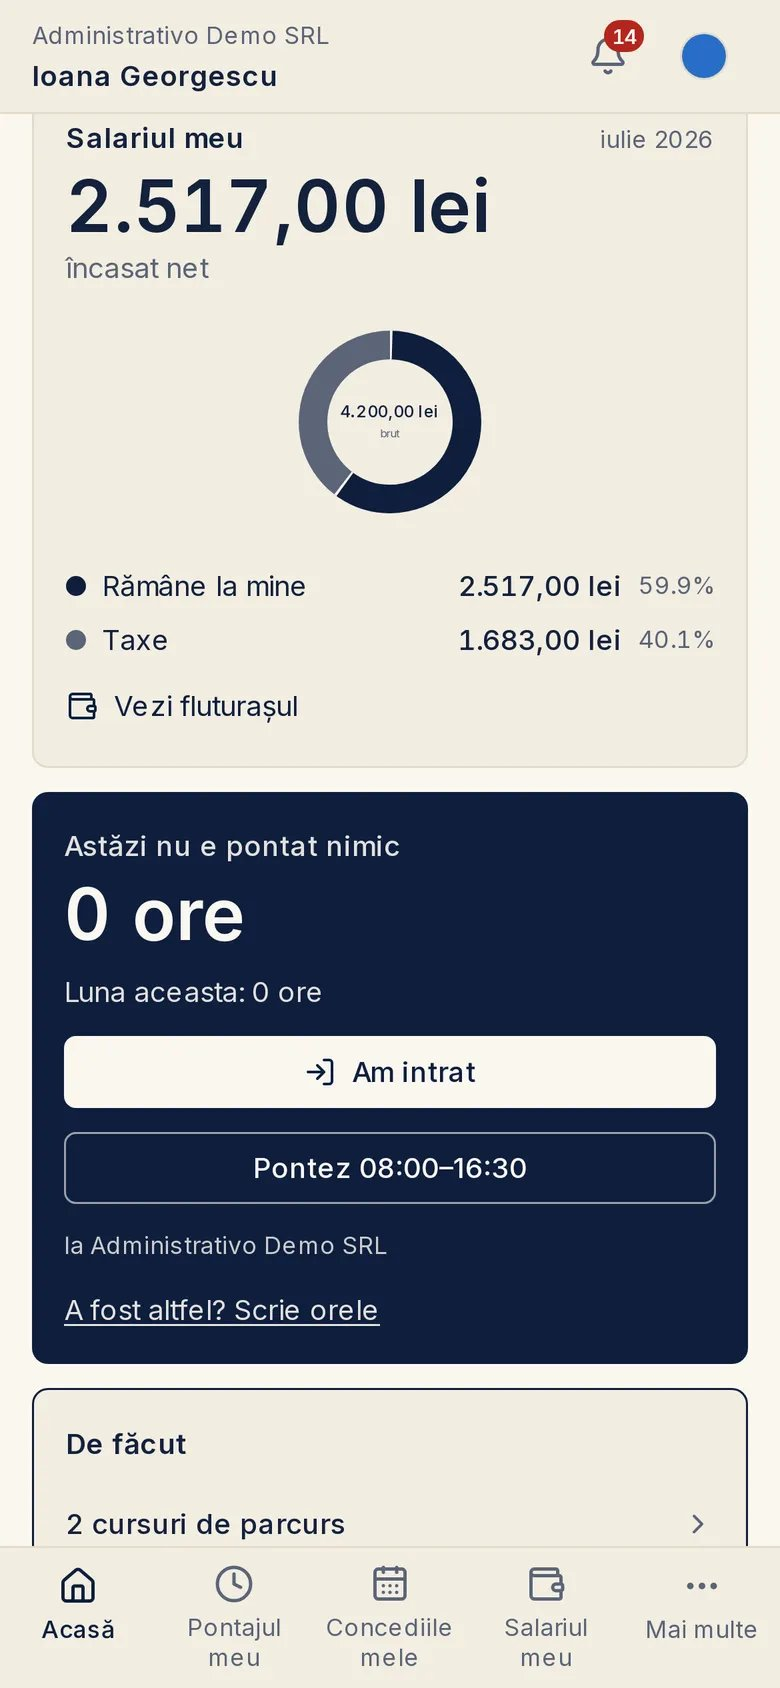
\includegraphics[height=3.0cm]{capturi/portal-pontare}\hspace{10pt}%
  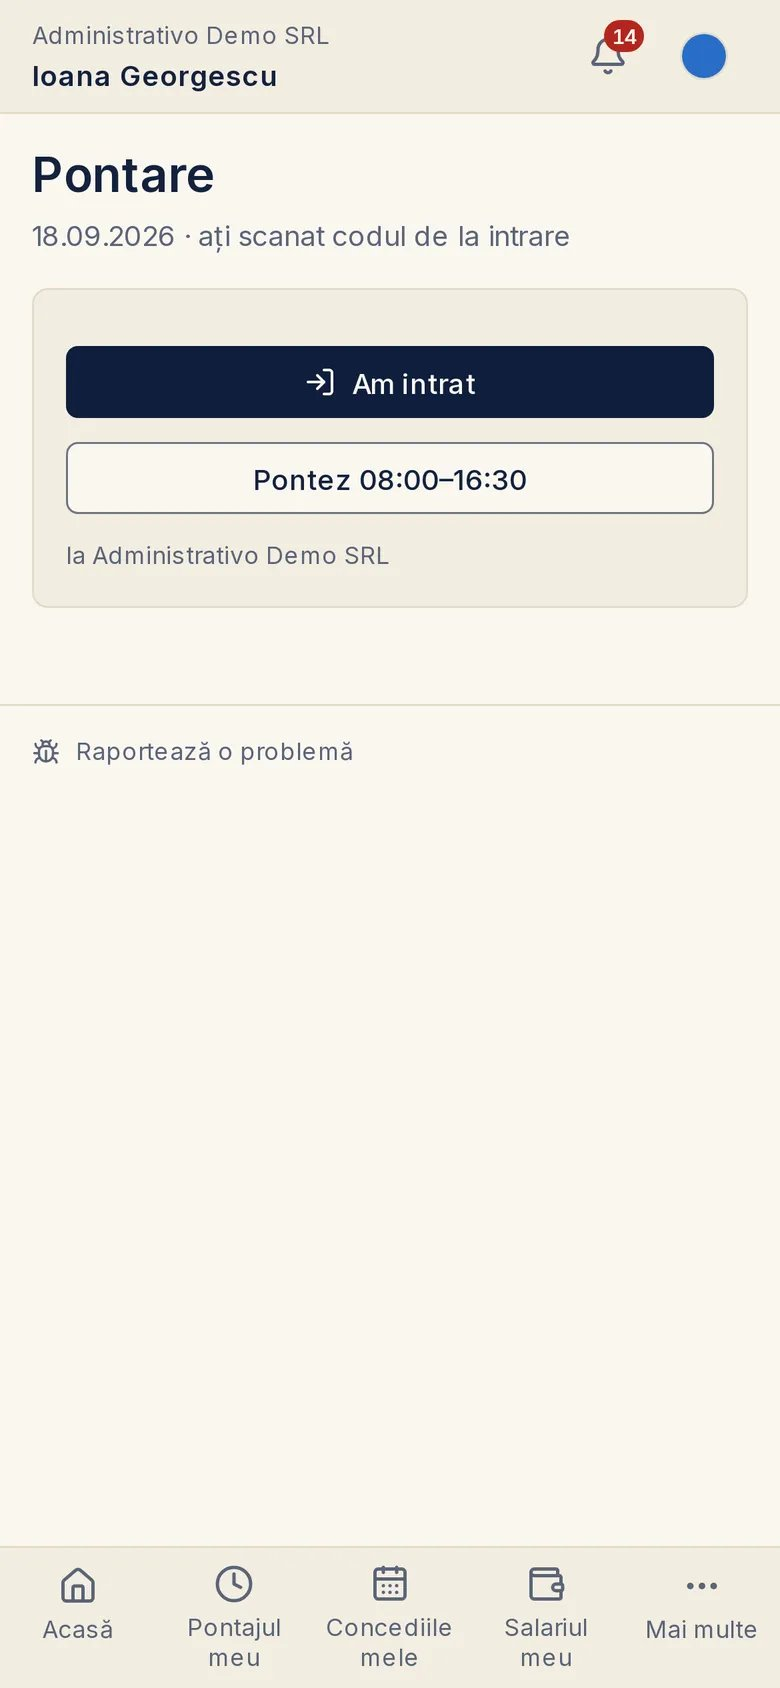
\includegraphics[height=3.0cm]{capturi/portal-scanare}}

% =====================================================================
%  REGES-ONLINE — fără captură
% =====================================================================
\modul{REGES-Online — contractele, transmise la ITM din aplicație}{hr extins}{%
  Fiecare eveniment din viața unui contract — angajare, modificare, suspendare,
  încetare — are termenul lui legal, iar amenda e \textbf{per salariat}. Mesajul se
  compune din fișa angajatului și pleacă direct la Inspecția Muncii.}{%
  \pct{stream}{Evenimente din fișă, concedii și pontaj}\par\vspace{2pt}
  \pct{calendar-day}{Termenul fiecărui eveniment, cu temeiul legal}\par\vspace{2pt}
  \pct{check-double}{Verificare înainte de trimitere, pe înțeles}\par\vspace{2pt}
  \pct{exchange-alt}{Trimis prin interfața REGES, cu răspunsul ITM}\par\vspace{2pt}
  \pct{percent}{Sporurile firmei, în nomenclatorul REGES}\par\vspace{2pt}
  \pct{bell}{Alertă pentru evenimentele netransmise}}{%
  \pctv{check}{\textbf{Termenul legal nu se mai ratează}}\par\vspace{4pt}
  \pctv{check}{\textbf{Nu se mai completează de două ori}, în două programe}\par\vspace{4pt}
  \pctv{check}{\textbf{Respingerea vine explicată în română}, nu ca un cod}\par\vspace{4pt}
  \pctv{check}{\textbf{Fiecare transmisie are dovadă} și răspuns păstrat}}

% =====================================================================
%  INTEGRARE ANGAJAȚI
% =====================================================================
\modulcaptura{Integrare angajați — prima săptămână, fără nimic uitat}{hr extins}{%
  Lista primei săptămâni devine un obiect cu stare: responsabil și termen pe
  fiecare pas, iar pașii cu dovadă nu se bifează fără ea.}{%
  \pct{copy}{Șabloane scrise o dată, refolosite}\par\vspace{2pt}
  \pct{user-check}{Responsabil și termen pe fiecare pas}\par\vspace{2pt}
  \pct{file-upload}{Dovada se încarcă și rămâne pe pas}\par\vspace{2pt}
  \pct{graduation-cap}{Cursul parcurs bifează singur pasul}\par\vspace{2pt}
  \pct{mobile-alt}{Omul nou își vede pașii în portal}}{%
  \benef{\textbf{Nimeni nu începe} fără laptop, cont și instruire}
  \benef{\textbf{Aceeași primire} pentru fiecare om}
  \benef{\textbf{Dovadă} că pasul obligatoriu s-a făcut}}{%
  \captura{onboarding}}

% =====================================================================
%  CURSURI
% =====================================================================
\modulcaptura{Cursuri — formarea internă și dovada ei}{hr extins}{%
  Lecțiile au materiale cu versiuni: versiunea veche rămâne, cu cine a parcurs-o.
  Cursul ajunge la oameni prin reguli, nu om cu om.}{%
  \pct{book}{Lecții cu materiale versionate}\par\vspace{2pt}
  \pct{chart-line}{Progres raportat pe măsură ce omul citește}\par\vspace{2pt}
  \pct{signature}{Lecția se semnează la final}\par\vspace{2pt}
  \pct{clipboard-check}{Test cu prag și rezultat păstrat}\par\vspace{2pt}
  \pct{sitemap}{Atribuire pe departament sau funcție}\par\vspace{2pt}
  \pct{hourglass-half}{Valabilitate și scadență de reînnoire}}{%
  \benef{\textbf{Se vede instantaneu} cine e restant}
  \benef{\textbf{Restanța ajunge la om}, în portal}
  \benef{\textbf{Dovadă de instruire} pentru control}}{%
  \captura{courses}}

% =====================================================================
%  SSM ȘI PSI
% =====================================================================
\modulcaptura{SSM și PSI — nimic nu expiră neobservat}{hr extins}{%
  O matrice: oamenii pe verticală, instruirile pe orizontală. „Niciodată făcută"
  nu se confundă cu „expirată" — la un control, diferența contează.}{%
  \pct{chalkboard-teacher}{Instruiri: introductivă, la post, periodică}\par\vspace{2pt}
  \pct{user-md}{Fișa de aptitudine medicală, cu termen}\par\vspace{2pt}
  \pct{hard-hat}{Echipament de protecție, predat nominal}\par\vspace{2pt}
  \pct{id-badge}{Autorizații nominale, cu scadență}\par\vspace{2pt}
  \pct{fire-extinguisher}{Stingătoare și verificări PSI}\par\vspace{2pt}
  \pct{ambulance}{Registrul accidentelor de muncă}}{%
  \benef{\textbf{Semaforul se aprinde} înainte de termen}
  \benef{\textbf{Dosar gata pentru ITM}, în orice zi}
  \benef{\textbf{Omul își vede instruirile} pe telefon}}{%
  \captura{ssm}}

% =====================================================================
%  EVALUĂRI
% =====================================================================
\modulcaptura{Evaluări — discuția anuală, pe criterii, nu pe impresii}{hr extins}{%
  Șablonul e al firmei: criterii, ponderi, scală. Evaluarea finalizată nu se mai
  modifică tăcut — redeschiderea lasă urmă.}{%
  \pct{sliders-h}{Șabloane cu criterii ponderate și scală}\par\vspace{2pt}
  \pct{copy}{Șablonul se duplică pentru anul următor}\par\vspace{2pt}
  \pct{star}{Scor calculat din criterii și ponderi}\par\vspace{2pt}
  \pct{comments}{Observații pe fiecare criteriu}\par\vspace{2pt}
  \pct{lock}{Finalizare și redeschidere cu urmă}\par\vspace{2pt}
  \pct{history}{Istoricul evaluărilor, pe angajat}}{%
  \benef{\textbf{Discuție pe date}, nu pe ultima lună}
  \benef{\textbf{Istoricul rămâne} când pleacă managerul}
  \benef{\textbf{Aceleași criterii} pe aceeași funcție}}{%
  \captura{evaluations}}

% =====================================================================
%  KPI-URI
% =====================================================================
\modulcaptura{KPI-uri — ținte scrise, pentru fiecare om}{hr extins}{%
  Trei lucruri care de obicei se amestecă, ținute separat: ce se măsoară, ținta
  fiecărui om și realizarea lunii. O lună închisă nu se mai rescrie.}{%
  \pct{list-ol}{Seturi de indicatori, cu unitate și sens}\par\vspace{2pt}
  \pct{bullseye}{Ținta pusă pe funcție, ajustată pe om}\par\vspace{2pt}
  \pct{calendar-alt}{Luna: deschisă, completată, închisă}\par\vspace{2pt}
  \pct{tachometer-alt}{Scor pe angajat, din realizări}\par\vspace{2pt}
  \pct{archive}{Setul vechi se arhivează, nu se șterge}\par\vspace{2pt}
  \pct{mobile-alt}{Omul își vede luna în lucru, în portal}}{%
  \benef{\textbf{Omul știe} pe ce e măsurat}
  \benef{\textbf{Evaluarea nu pornește} de la zero}
  \benef{\textbf{Ținta de atunci} rămâne scrisă}}{%
  \captura{kpi}}

% =====================================================================
%  PARC AUTO
% =====================================================================
\modulcaptura{Parc auto — scadențele, foile de parcurs, consumul}{resurse și logistică}{%
  Fiecare vehicul are termenele lui, cu semafor aprins înainte de scadență.
  Istoricul rămâne pe mașină, nu pe șofer.}{%
  \pct{car}{ITP, RCA, rovinietă, tahograf, licență}\par\vspace{2pt}
  \pct{route}{Foi de parcurs, cu kilometrajul}\par\vspace{2pt}
  \pct{gas-pump}{Alimentări și consum, comparat cu bonurile}\par\vspace{2pt}
  \pct{exclamation-triangle}{Anomalii: kilometraj în salt, consum aberant}\par\vspace{2pt}
  \pct{user-check}{Șeful de echipă aprobă foile oamenilor lui}}{%
  \benef{\textbf{Nicio scadență} de ITP sau RCA pierdută}
  \benef{\textbf{Consumul aberant} se vede imediat}
  \benef{\textbf{Istoricul} nu se rupe la schimbarea șoferului}}{%
  \captura{fleet}}

% =====================================================================
%  MENTENANȚĂ
% =====================================================================
\modulcaptura{Mentenanță — revizia înainte de defecțiune}{resurse și logistică}{%
  Oricine deschide o sesizare, pe orice echipament, iar ea primește un
  responsabil. Reviziile se planifică pe dată sau pe contor.}{%
  \pct{cogs}{Fișă de echipament, cu autorizații ISCIR}\par\vspace{2pt}
  \pct{bullhorn}{Sesizări de la oricine, triate și atribuite}\par\vspace{2pt}
  \pct{calendar-check}{Planuri de revizie pe dată sau pe contor}\par\vspace{2pt}
  \pct{tachometer-alt}{Citiri de contor, cu scadența calculată}\par\vspace{2pt}
  \pct{tools}{Intervenții, cu cost de piese și manoperă}}{%
  \benef{\textbf{Revizia se face} înainte de defecțiune}
  \benef{\textbf{Sesizarea ajunge în sistem}, nu pe chat}
  \benef{\textbf{Autorizația ISCIR} nu expiră neobservat}}{%
  \captura{maintenance}}

% =====================================================================
%  INVENTAR
% =====================================================================
\modulcaptura{Inventar — ce deține firma și cine are fiecare lucru}{resurse și logistică}{%
  Obiectul intră în stoc, se predă, se returnează sau se casează. Primirea o
  confirmă angajatul — așa devine lista o dovadă.}{%
  \pct{boxes}{Fișă per obiect: cod, serie, stare}\par\vspace{2pt}
  \pct{user-tag}{Predare nominală, cu data ei}\par\vspace{2pt}
  \pct{file-signature}{Proces-verbal de predare-primire}\par\vspace{2pt}
  \pct{clipboard-check}{Angajatul confirmă primirea din portal}\par\vspace{2pt}
  \pct{history}{Istoricul obiectului, până la casare}}{%
  \benef{\textbf{Nimic nu se pierde} la plecarea unui om}
  \benef{\textbf{Responsabilitate clară}, confirmată}
  \benef{\textbf{Inventarul se închide} într-o zi}}{%
  \captura{inventory}}

% =====================================================================
%  ANUNȚURI
% =====================================================================
\modulcaptura{Anunțuri — comunicarea internă, cu dovadă de citire}{resurse și logistică}{%
  Nu un e-mail din care nu știi cine l-a deschis: anunțul se publică pentru
  toată firma, iar citirea se înregistrează pe fiecare om.}{%
  \pct{pen}{Ciornă, apoi publicare cu data ei}\par\vspace{2pt}
  \pct{thumbtack}{Anunțurile importante, fixate sus}\par\vspace{2pt}
  \pct{bell}{În aplicație, în portal și pe telefon}\par\vspace{2pt}
  \pct{check-double}{Confirmare de citire, per angajat}\par\vspace{2pt}
  \pct{chart-pie}{Cine a citit și cine nu, pe nume}}{%
  \benef{\textbf{Dovadă} că informarea a fost citită}
  \benef{\textbf{Ajunge și la cei} fără e-mail de serviciu}
  \benef{\textbf{Nu mai există} „nu am știut"}}{%
  \captura{announcements}}

% =====================================================================
%  TICKETING IT
% =====================================================================
\modulcaptura{Ticketing IT — cererile colegilor, cu număr și răspuns}{resurse și logistică}{%
  Cererea capătă număr, responsabil și stare. Prioritatea nu se alege: se
  calculează din tipul cererii și din câți au aceeași problemă.}{%
  \pct{ticket-alt}{Software, hardware, defecțiuni, erori}\par\vspace{2pt}
  \pct{sort-amount-up}{Prioritate calculată; manual, doar cu motiv}\par\vspace{2pt}
  \pct{clone}{Duplicatele se leagă de tichetul inițial}\par\vspace{2pt}
  \pct{users}{Coada pe echipă, nu pe persoană}\par\vspace{2pt}
  \pct{comments}{Discuție pe tichet, cu istoricul păstrat}\par\vspace{2pt}
  \pct{mobile-alt}{Deschis și urmărit din portal}}{%
  \benef{\textbf{Nicio cerere pierdută}}
  \benef{\textbf{Nimeni nu mai sună} să întrebe de stare}
  \benef{\textbf{Se vede ce se strică des}}}{%
  \captura{ticketing}}

% =====================================================================
%  SALARIZARE
% =====================================================================
\modulcaptura{Salarizare — din pontajul închis, până la bancă}{financiar}{%
  Calculul pornește din luna de pontaj închisă, cu desfășurător pe fiecare
  linie. Cotele sunt ale firmei, cu data de la care se aplică.}{%
  \pct{calculator}{Brut, contribuții, impozit, net, pe linii}\par\vspace{2pt}
  \pct{percent}{Sporuri, prime, avantaje, scutiri fiscale}\par\vspace{2pt}
  \pct{exclamation-triangle}{Avertisment lângă cifra neobișnuită}\par\vspace{2pt}
  \pct{file-code}{D112 în XML, validat înainte de depunere}\par\vspace{2pt}
  \pct{university}{Fișier de plată SEPA și notă contabilă}\par\vspace{2pt}
  \pct{gavel}{Popriri în limitele art.~729 CPC}}{%
  \benef{\textbf{Nimic retastat} din pontaj}
  \benef{\textbf{Erorile D112} se află înainte}
  \benef{\textbf{Fluturașul} ajunge în portal}}{%
  \captura{payroll}}

% =====================================================================
%  DEPLASĂRI ȘI DIURNE
% =====================================================================
\modulcaptura{Deplasări și diurne — de la ordin la decont}{financiar}{%
  Ordin, etape pe țări, decont. Diurna externă se numără de la ora plecării, iar
  partea neimpozabilă se calculează separat.}{%
  \pct{plane}{Deplasări interne și externe, pe etape}\par\vspace{2pt}
  \pct{globe-europe}{Baremul fiecărei țări, la vedere}\par\vspace{2pt}
  \pct{clock}{Ferestre de 24 h sau zile calendaristice}\par\vspace{2pt}
  \pct{balance-scale}{Politica firmei, cu plafonul legal arătat}\par\vspace{2pt}
  \pct{calculator}{Partea neimpozabilă, separată}\par\vspace{2pt}
  \pct{user-check}{Șeful aprobă, fără să modifice cifrele}}{%
  \benef{\textbf{Aceeași regulă} pentru toți}
  \benef{\textbf{Intră în salarizare} gata separată}
  \benef{\textbf{Omul își face singur} ordinul}}{%
  \captura{per_diem}}

% =====================================================================
%  RAPOARTE
% =====================================================================
\modulcaptura{Rapoarte — costul cu personalul, într-un ecran}{financiar}{%
  Cifrele vin din ce a trecut deja prin aprobare — salarizarea calculată,
  pontajul închis — nu dintr-o copie în Excel.}{%
  \pct{chart-bar}{Venit brut și net, pe an și pe lună}\par\vspace{2pt}
  \pct{coins}{Cost total angajator, lună de lună}\par\vspace{2pt}
  \pct{chart-pie}{Unde se duce costul: net, taxe, contribuții}\par\vspace{2pt}
  \pct{utensils}{Tichete de masă acordate}\par\vspace{2pt}
  \pct{clock}{Ore suplimentare și zile de concediu}\par\vspace{2pt}
  \pct{user}{Același tabel, pe fiecare angajat}}{%
  \benef{\textbf{Decizia se ia} pe cifra din sistem}
  \benef{\textbf{Corectura la sursă} schimbă raportul}
  \benef{\textbf{Fără export} de prelucrat}}{%
  \captura{rapoarte}}

% =====================================================================
%  ASISTENT AI — fără captură
% =====================================================================
\modul{Asistent AI — întrebări în română, despre aplicație și date}{transversal}{%
  O bulă de conversație în colțul ecranului. Omul știe ce vrea, dar nu știe unde
  se face: asistentul răspunde și, când răspunsul e un ecran, duce direct acolo.
  Vede exact ce ai voie să vezi tu.}{%
  \pct{comments}{Întrebare în română, răspuns scris pe loc}\par\vspace{2pt}
  \pct{compass}{Te duce direct în ecranul căutat}\par\vspace{2pt}
  \pct{database}{Aceleași date, prin aceleași reguli ca aplicația}\par\vspace{2pt}
  \pct{shield-alt}{Fără permisiuni proprii: ajunge unde ajunge omul}\par\vspace{2pt}
  \pct{toggle-off}{Se oprește de tot, pe firmă, dintr-un comutator}}{%
  \pctv{check}{\textbf{„Câte zile de concediu mai am?"} — răspuns în câteva secunde}\par\vspace{4pt}
  \pctv{check}{\textbf{Omul nou găsește ecranul} fără să întrerupă un coleg}\par\vspace{4pt}
  \pctv{check}{\textbf{Nicio cale ocolită}: același refuz ca pe ecran}\par\vspace{4pt}
  \pctv{check}{\textbf{Nu învață din datele firmei} și nu antrenează nimic pe ele}}

% =====================================================================
%  FINAL / CONTACT
% =====================================================================
\begin{frame}[plain]
  \begin{tikzpicture}[remember picture,overlay]
    \fill[brandNavy] (current page.south west) rectangle (current page.north east);
    \fill[brandBlue,opacity=0.20] ([xshift=-2.6cm,yshift=-1.8cm]current page.east) circle (4.4cm);
    \fill[brandTeal,opacity=0.13] ([xshift=-4.6cm,yshift=2.6cm]current page.east) circle (3.0cm);
    \draw[brandTeal,opacity=0.28,line width=0.7pt]
      ([xshift=-2.6cm,yshift=-1.8cm]current page.east) circle (5.5cm);

    \node[anchor=north west,align=left] at ([xshift=1.45cm,yshift=-2.3cm]current page.north west) {%
      \begin{minipage}{13.4cm}
        \raggedright
        {\titlufont\bfseries\fontsize{24}{28}\selectfont\color{white} Prima lună e gratuită.}\par
        \vspace{9pt}
        {\color{brandLine}\small
         Fără taxă de înrolare și fără card. Pornim doar modulele de care aveți
         nevoie, vă importăm datele și vă arătăm cum se lucrează. Celelalte se pot
         porni oricând, fără reinstalare.}
        \par\vspace{11pt}
        {\color{white}\footnotesize
         \faIcon{building}~~\textbf{WISELEARNING SRL} \quad
         \faIcon{phone-alt}~~\textbf{(+40) 767 991 625} \quad
         \faIcon{envelope}~~\textbf{contact@administrativo.ro}}
        \par\vspace{5pt}
        {\color{brandLine}\scriptsize
         \faIcon{globe}~~administrativo.ro \quad\textcolor{brandTeal}{\textbullet}\quad
         Str. Metalurgiei nr. 2, Timișoara, jud. Timiș \quad\textcolor{brandTeal}{\textbullet}\quad
         CIF 50321210}
      \end{minipage}};

    \node[anchor=south west,align=left] at ([xshift=1.5cm,yshift=0.95cm]current page.south west) {%
      \begin{minipage}{13.2cm}
        {\color{brandTeal}\rule{2.2cm}{2pt}}\par
        \vspace{9pt}
        {\color{white}\scriptsize
          \faIcon{calendar-check}~~Demonstrație de 30 de minute \quad\textcolor{brandTeal}{\textbullet}\quad
          \faIcon{infinity}~~Modulele noi, incluse \quad\textcolor{brandTeal}{\textbullet}\quad
          \faIcon{headset}~~Suport non-stop, inclus}
      \end{minipage}};
  \end{tikzpicture}
\end{frame}

\end{document}
